\chapter{Exploratory Analysis}
First part of the analysis is to explore the different attributes in the data, in order to detect possible patterns or correlations. The exploratory analysis is also used to get an understanding of data and its behaviour. Hence, this chapter is about visualizing the different attributes focusing on their influence on the heat consumption. As the heat in each house is turned off in the summer period, data is segmented such that the summer period is excluded from the data used for modeling. \\

\section{Examination of the Heat Consumption}
\noindent To get an overview of the heat consumption for each house, the daily average heat consumption for each house is investigated. \cref{fig: daily_cons} shows the daily average consumption for all the houses and the daily consumption of two houses - one that follows the trend and one that deviates. It can be seen that the slopes around the summer months are close to 0. As mentioned, the data in focus in this project is where the heat is turned on, hence the period where the heat consumption is close to 0 needs to be removed. Exactly how this is done will be explained and discussed in the data segmentation section. All three plots show some unusual high data points around April 2018. This can be due to the fact that is was snowing in Denmark at that time which is supported by the article found in \cite{vejr2018}. \\
\begin{figure}
    \centering
    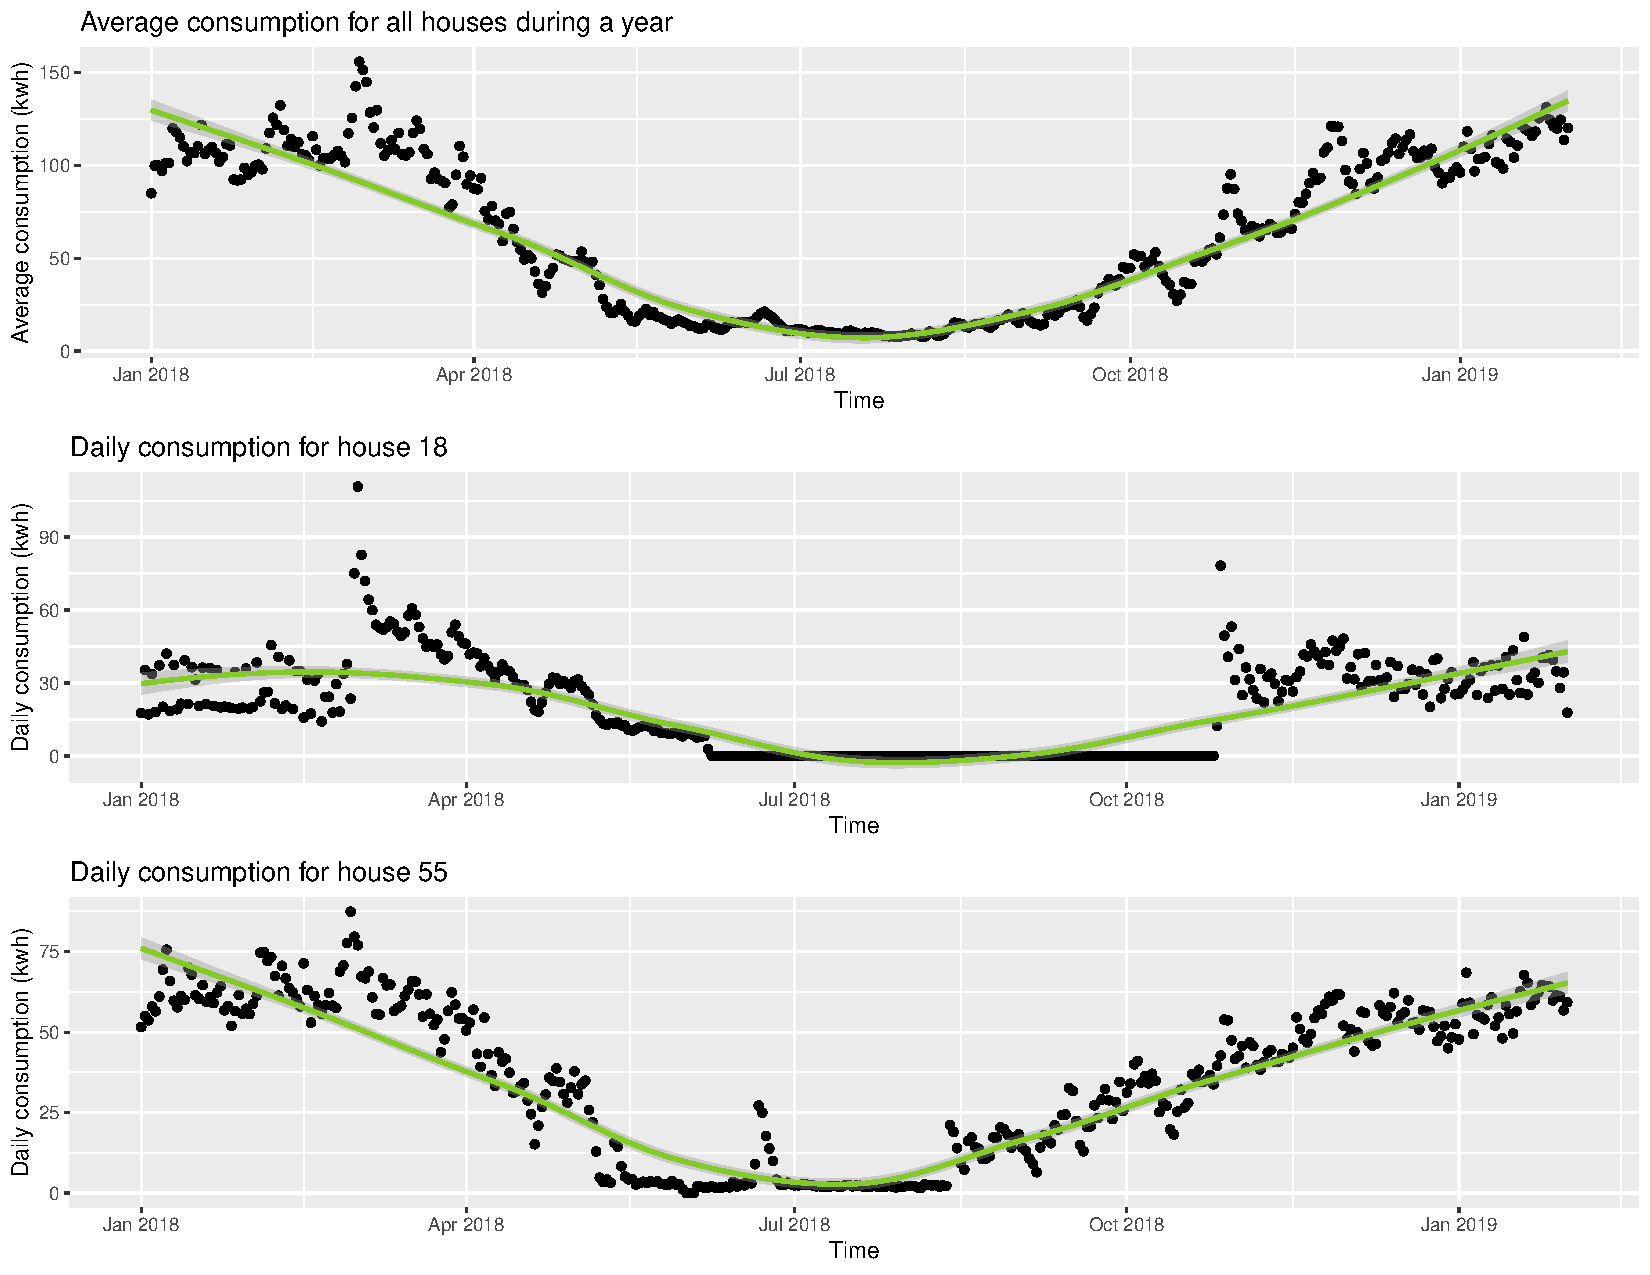
\includegraphics[width=1.\textwidth]{../../../figures/avg_daily.pdf}
    \caption{Daily consumption during a year (2018). The top plot shows the average consumption for all the houses. The plot in the middle shows an example of a house that follows the trend and the last plot shows a house that deviates from the trend}
    \label{fig: daily_cons}
\end{figure}

\noindent The remaining attributes from the house data is examined through a scatterplot shown in \cref{fig: housepairs} and \cref{fig: house_attri}, in order to find possible linear relationships with the consumption. There are clear linear relationships between the consumption and the flow, the volume, the cooling degree and the temperature going in respectively. It is expected that the consumption depends linearly on the volume and cooling degree, cf. the main equation given in \cref{eq: Q_heat}. The relationships between consumption and the flow and volume are quite similar which is in line with the description of the two attributes given in \cref{tab: housedata}. \textcolor{blue}{Det varme vand der kommer ud af systemet afhænger af hvor meget man bruger. Det ses, at hvis det vand der kommer ud er meget varmt, så er det fordi man ikke har brugt det, eller trukket sådan varmeforbrug ud af det.}
\begin{figure}
    \centering
    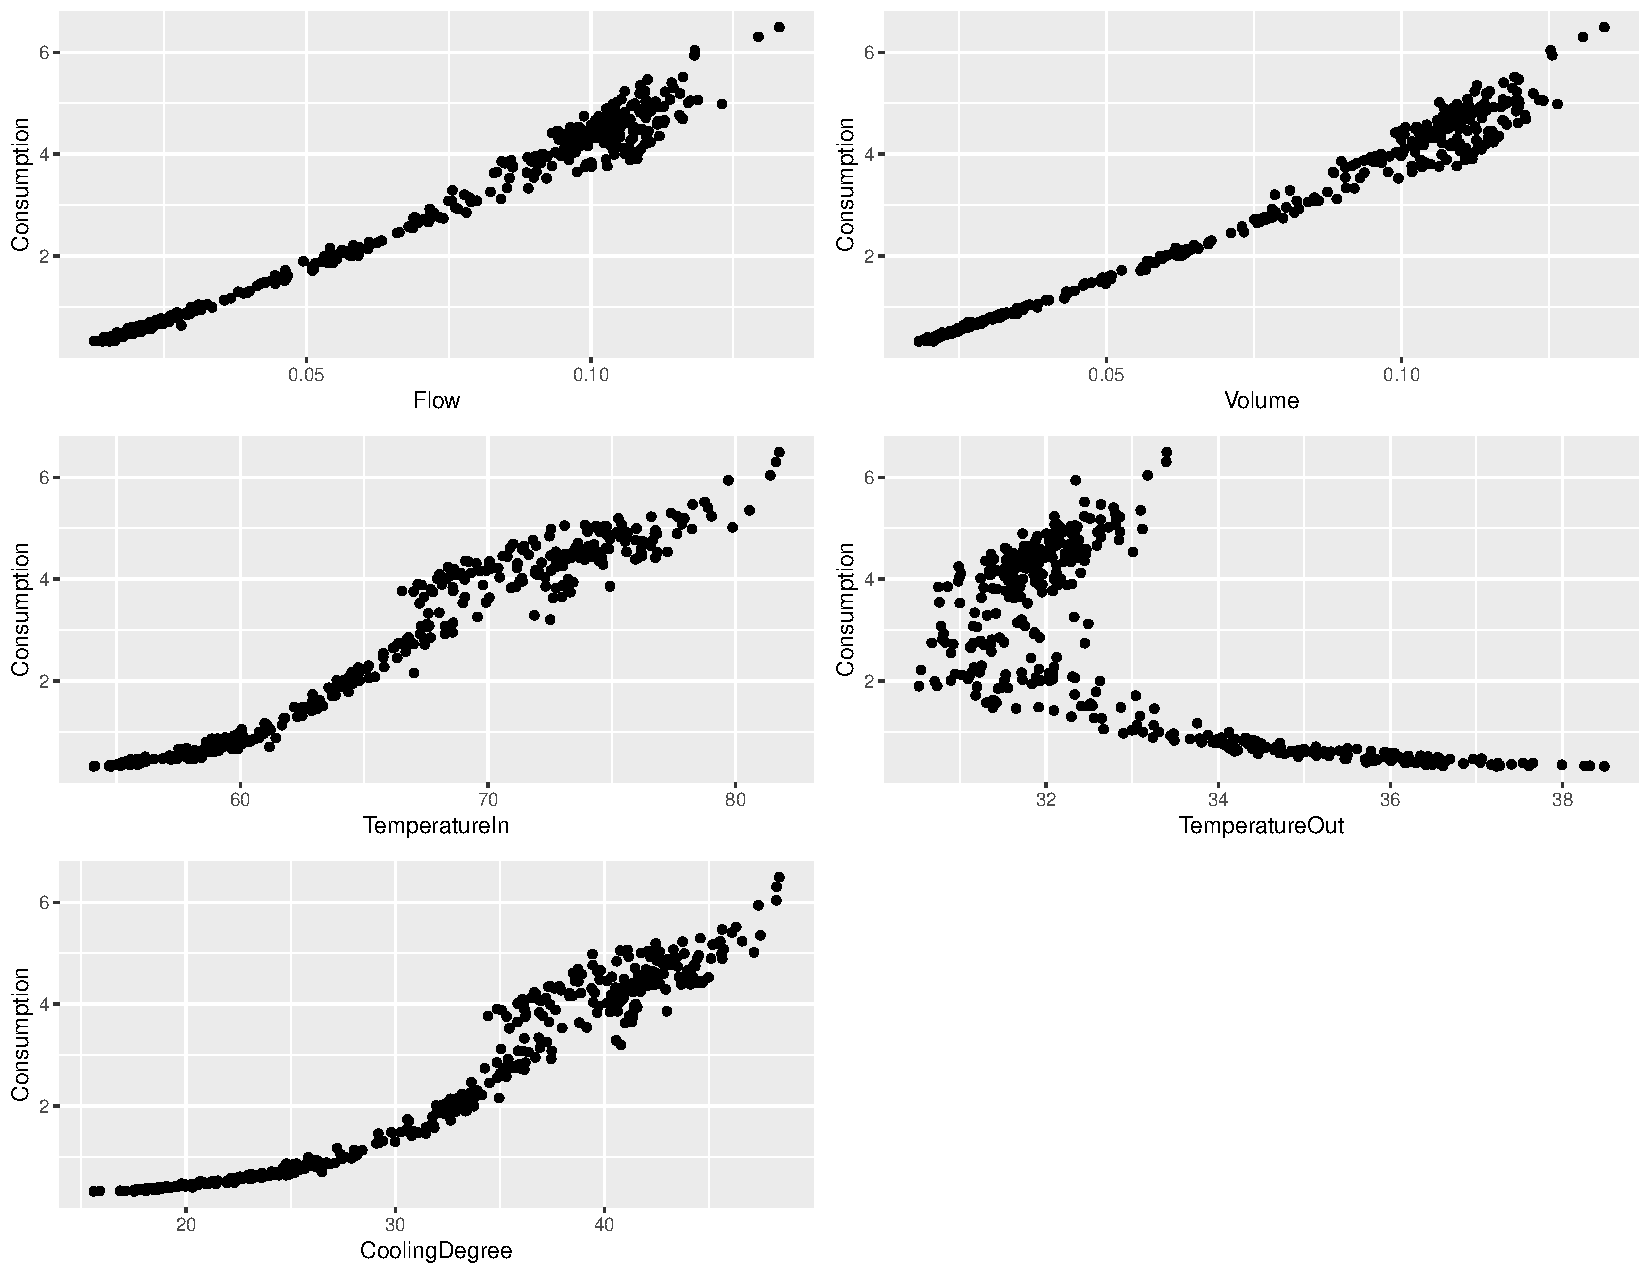
\includegraphics[width=1.\textwidth]{../../../figures/housepairs.pdf}
    \caption{Scatterplots of the daily values of relevant house attributes. There are clear linearly dependencies between \texttt{Consumption} and e.g. \texttt{Flow}} 
    \label{fig: housepairs}
\end{figure}


%\noindent Figure \ref{fig: house_attri} clearly shows that the consumption is close to 0 in the summer period.  
%\textcolor{red}{Pairs af gennemsnitlig house data - vi ser en masse sammenhænge mellem de forskellige attributer. Vi kan se at CoolingDegree skal være over 25, før at varmeforbruget stiger.}
%\textcolor{red}{CoolingDegree begynder at stige et stykke tid før flowet stiger, hvilket hænger godt sammen med at når man fx tænder en radiator så stiger CoolingDegree. De efterfølgende radiatorer man tænder øger volumnet.} \\

\textcolor{blue}{\noindent It is already known that there is a dependency between the heat consumption and the time of the year. During the summer period there is almost no consumption. The consumption in this period is probably mostly tap water. The next important thing is the relation between temperature and consumption. High temperatures tend to imply a higher consumption. And the reason why the consumption depends so clearly on the time of year can be assumed to that certain periods have similar temperature levels. It can also be seen that there is a correlation between dewpoint and consumption. This can be due to the correlation between dewpoint and temperature.}


\subsection{Weather data}
The weather data is also examined through scatterplots given in \cref{fig: weatherpairs} and \cref{fig: weather_cons}. in order to detect dependencies between the average consumption of the houses and the weather attributes. The temperature outside has a high 
\begin{figure}
    \centering
    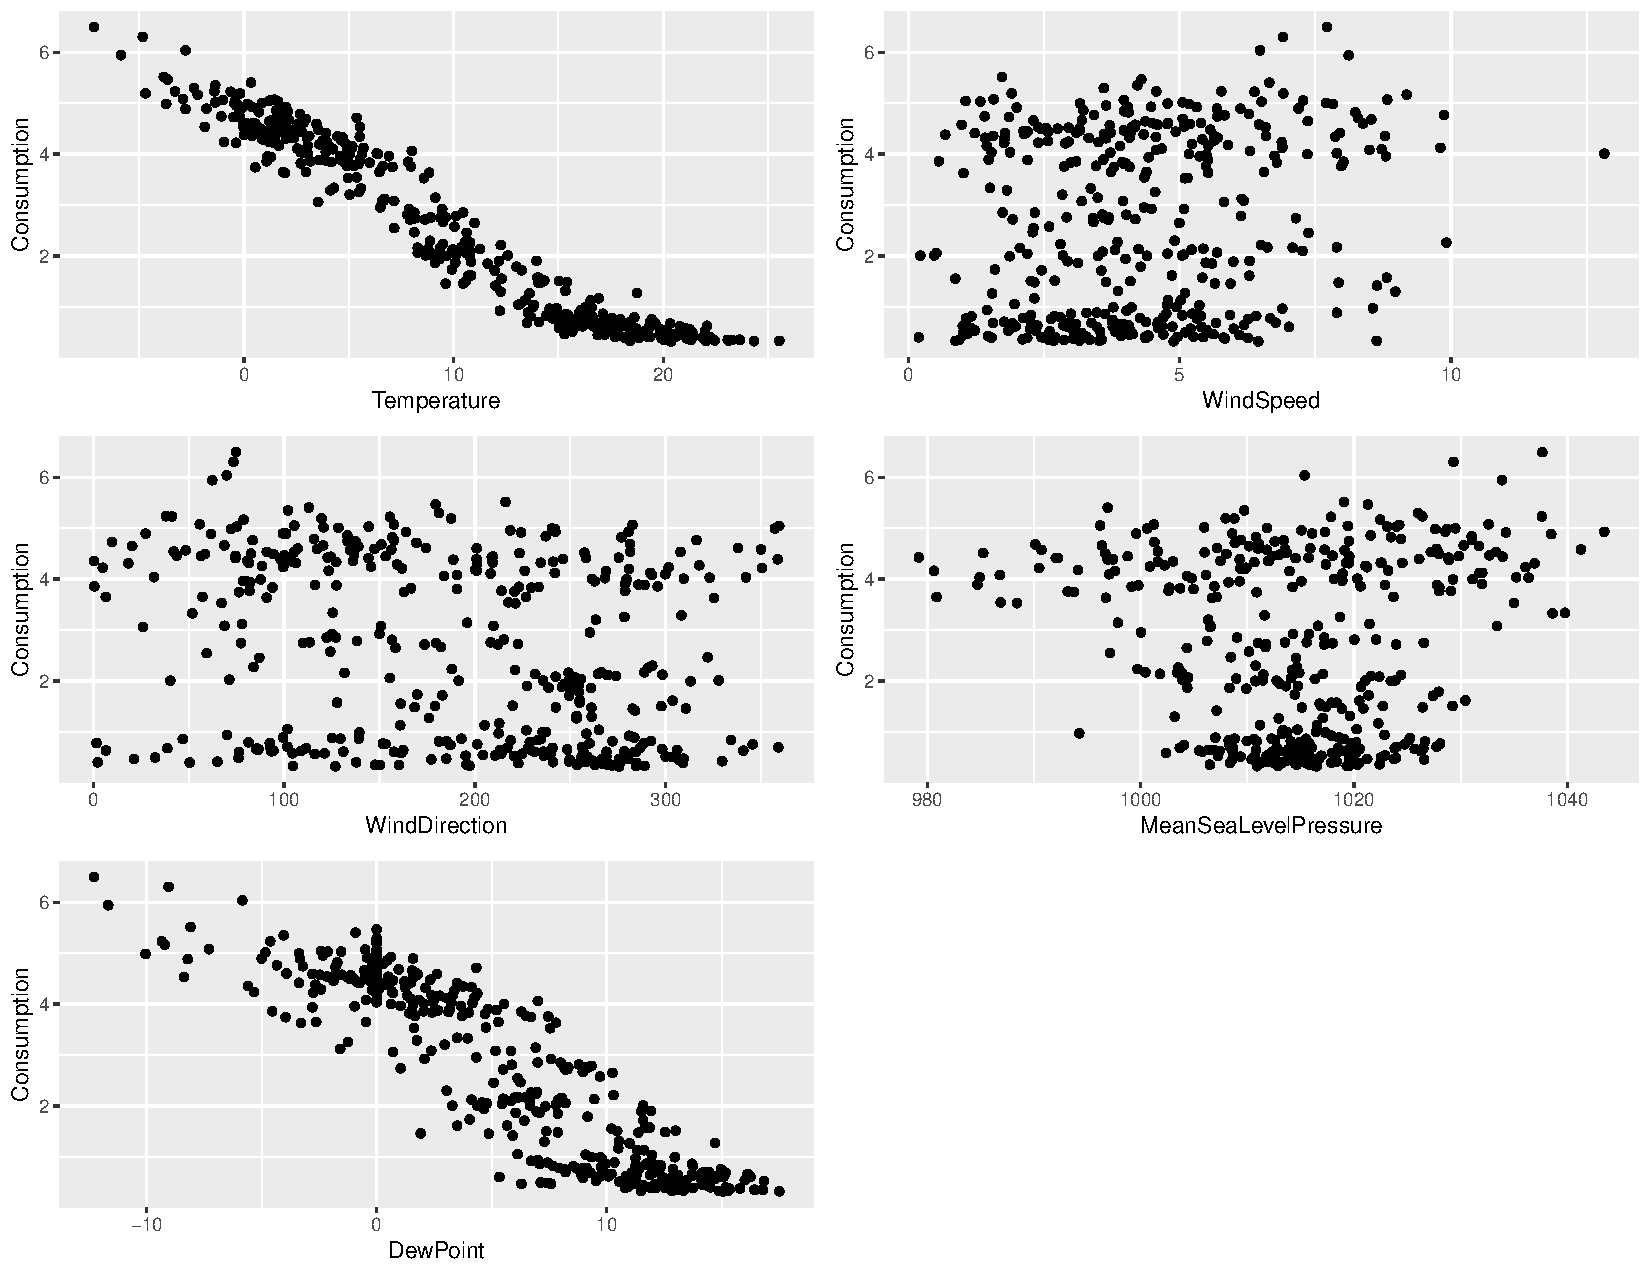
\includegraphics[width=1.\textwidth]{../../../figures/weatherpairs.pdf}
    \caption{Scatterplots of the daily values of relevant weather attributes. There are clear linearly dependencys between \texttt{Consumption} and \texttt{Temperature} as was expected}
    \label{fig: weatherpairs}
\end{figure}

\subsection{BBR data}
Presumably, the BBR data has influence on the heat consumption in particular the total area and year of construction. \textcolor{red}{Mangler lidt her.} \\

\noindent The average of the heat consumption for each house is found/determined for the winter period. By dividing the average consumption with the total area of the house the consumption pr. $m^2$ is calculated. Figure \ref{fig: byggeaar} shows the year of construction and the consumption for each of the houses. The year of construction is here determined by either the year of construction or the year of the latest reconstruction of a house. 
\begin{figure}
    \centering
    \includegraphics[width=1.\textwidth]{../../../figures/byggeår.eps}
    \caption{Plot showing the year of construction and the average consumption pr. $m^2$ for each house. It is clearly seen that there is a tendency that the later a house is built or reconstructed, the better is the insulation of the house}
    \label{fig: byggeaar}
\end{figure}

\noindent Figure \ref{fig: byggeaar} clearly shows that the later a house is constructed (or reconstructed), the better is the insulation of the house as the consumption decreases with the year of construction. Furthermore, there is a clear outlier in the figure which has a remarkable high consumption pr. $m^2$. When looking up the house in the BBR data, it is seen that the outlier is an apartment of 61 $m^2$ build in 1920.  

\section{Multicollinearity}
Multicollinearity occurs when two or more explanatory variables are highly correlated. In linear regression, multicollinearity \textcolor{red}{\dots} Multicollinearity can be investigated by calculating the correlation using the function \texttt{cor()} in \texttt{R}.\\

\noindent Figure \ref{fig: weather_cons} clearly shows that there is a high correlation between \texttt{Temperature} and \texttt{Dewpoint}. The exact correlation between the two attributes is calculated at 0.936, hence it is decided to remove \texttt{Dewpoint}. Furthermore, it is assumed that \texttt{Radiation} is a replacement for the attributes describing the sun, namely \texttt{Condition} and \texttt{SunHour}. This is the basis for expecting a correlation between the radiation and the sun attributes. Figure \ref{fig: gg_cor} shows a plot of the correlation matrix between the abovementioned attributes.
\begin{figure}
    \centering
    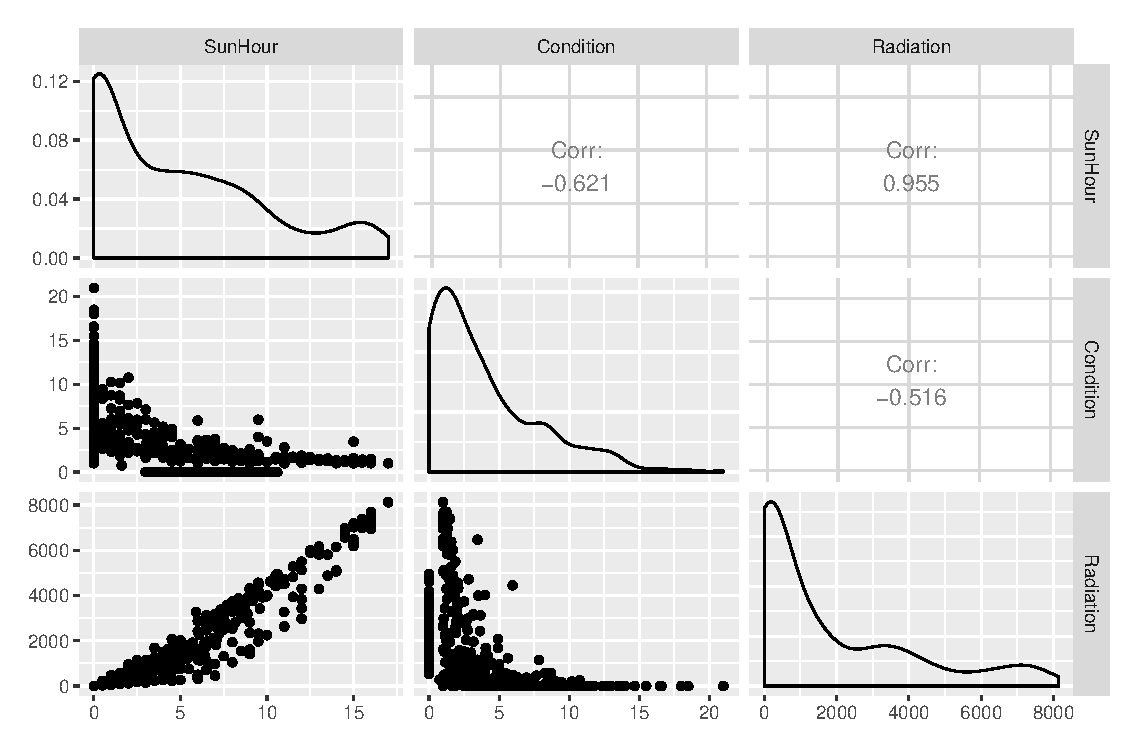
\includegraphics[width=1.\textwidth]{../../../figures/gg_cor.eps}
    \caption{Scatterplot showing the correlations between the three attributes \texttt{Condition}, \texttt{Radiation} and \texttt{SunHour}. It is clearly seen that the radiation and the sun hour are highly correlated}
    \label{fig: gg_cor}
\end{figure}
\noindent There is a high correlation between \texttt{Radiation} and \texttt{SunHour} at 0.955, thus \texttt{SunHour} is removed from the weather data set. \\
 
\noindent The complete data set used for modeling in chapter 4 can be seen in table \ref{tab: modeldata}. 
\begin{table}
    \centering
    \begin{tabular}{ll}
     \hline
     \textbf{Variable} & \textbf{Description} \\
    \hline
    \hline
    Date  &  End time and date for measurements. Hourly values.\\
    Temperature  &  Temperature outside in Degrees/C. \\
    WindSpeed  &  \\ 
    WindDirection  &  \\
    Condition  & \\
    MeanSeaLevelPressure & Avg. atmospheric pressure at mean sea level in mbar.\\
    PrecipitationProbability & Measure of the probability that precipitation will occur. \\
    Observation & The number of observations for each day for each house.\\
    Consumption & CoolingDegree times Volume from House data \\
    Holiday & A categorical attribute with 6 levels: Working day, \\ & Weekend, Autumn break, Christmas break, \\ & Winter break and Spring break.\\
    \hline
    \end{tabular}
    \caption{Attributes used for modeling}
    \label{tab: modeldata}
\end{table}   

\section{Data segmentation}
Since one of the focuses of this paper is to estimate how much energy a house uses for heating
depending on different outside temperatures, it is important to distinguish between when the house
is actually being heated, and when the water is just being used for tap water consumption. If the
inhabitants are not home for a longer period, there will probably be low consumption, even though
it might be cold outside. This does not necessarily mean that the house is well isolated. And if
there is consumption in warm periods, it is likely to be tap water consumption, and not heating
The data can be seen as part of two different distributions. One where the heating is turned off,
 and one where it is turned on. In this section different approaches will be examined on how to
 distinguish between the two distributions.
The goal is to find some temperature, where it can be assumed that all data points below it belongs
to the distribution with heating turned on. Two approaches will be described below, together with
their pros and cons.

\subsection{Segmentation by piece-wise optimization}
The first approach is to make a linear regression on the data with two segments. A breakpoint
$\alpha$ is found, such that the SSE is as small as possible. The second segment is restricted to
being constant. This way the breakpoint illustrates when the consumption goes from being linearly
dependent on the temperature, to having a constant value. This method was tested on every available
house, where a new breakpoint was found for each house.

\noindent Figure \ref{fig: Consumption-PW} shows the regression for two different houses. On both houses the
line fits rather well with the low-temperature data points. But it is not very accurate around the breakpoint.
The house on the left shows very clearly, that the assumption that all points below the breakpoint belong to 
the distribution without heating, is not accurate. Even though this approach can easily take out a lot of data
where there is clearly no heating, it will in many cases set the breakpoint too high. The "tail" of the low
consumption distribution might still be included, causing a bias in the model, and some variation that is not
accounted for. The method is also not very robust. Depending on how the points are spread out, the breakpoint
is sometimes as high as 20 degrees, which is not desirable.
\begin{figure}
    \centering
    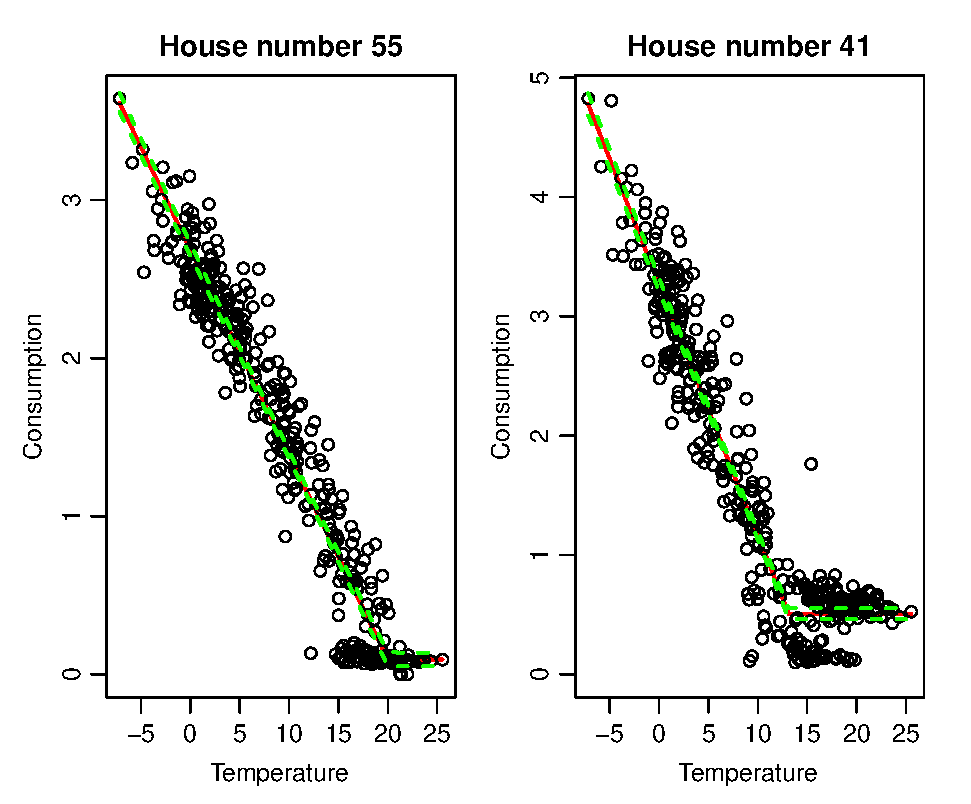
\includegraphics[width=0.8\textwidth]{../../../figures/Consumption-PW.eps}
    \caption{Piece-wise optimization of the consumption. The red line is the regression line and the green line is the confidence interval.}
    \label{fig: Consumption-PW}
\end{figure}


\subsection{Segmentation by significant deviations}
In the second approach, the data points are examined from high temperatures to low. First, all data points from
above 20 degrees are assumed to belong to the distribution without heating. If a data point is more than two
standard deviations above from the mean of this distribution, it is assumed to belong to the distribution with
heating. Now the data points are divided by temperature into one degree intervals. For each interval, starting
from above and moving down, all data points in that interval are examined. The last interval where at least
20\% of the data points are less than two standard deviations away, is chosen as the breakpoint of that house.
An example of the approach is seen on figure \ref{fig: Breakpoint}. On the left the data points are plotted with
standard deviations on the y-axis. The red line highlights the two standard devations. On the right there is a plot
showing how many of the data points that are outside the interval. Here, the red line shows the 80\% that determine
the breakpoint. The orange line shows the breakpoint.

This model is more robust than the first. It is more selective, and provides a good way to set the
breakpoint on the correct side of the mentioned "tail" that may occur at temperatures both with and without heating.
When comparing figure \ref{fig: Breakpoint} to figure \ref{fig: Consumption-PW}, one can see that this method sets
the breakpoint a bit lower, removing more points without heating. If the consumption data behaves badly, and chunks
of datapoints are low enough to be within the two standard deviation, then a lot of data can potentially be removed,
and there might be too little data left.

Until now the focus has been to find a breakpoint for every individual house. But it might be preferable to have a
single breakpoint all houses. This way the segmentation becomes more robust to houses with unforseen heat consumption.
Figure \ref{fig: AlphaHist} shows a histogram of the breakpoint values for every house in the data set. The global
breakpoint should be in the low end of the scale. It is better to remove data points that could have been used, than
to include too many points that belong to a different distribution with a different variation, which could make the
assumptions of the model worse. It would not be good to choose the minimum breakpoint, since that would be very
vulnerable. A single house with a very low breakpoint might make the model bad for all the other houses. So the
breakpoint that is chosen is the first quantile. As it is shown on the figure, this is $12$ degrees. All models in
the following sections will only be considering data where the temperature less than or equal to $12$ degrees.

\begin{figure}
    \centering
    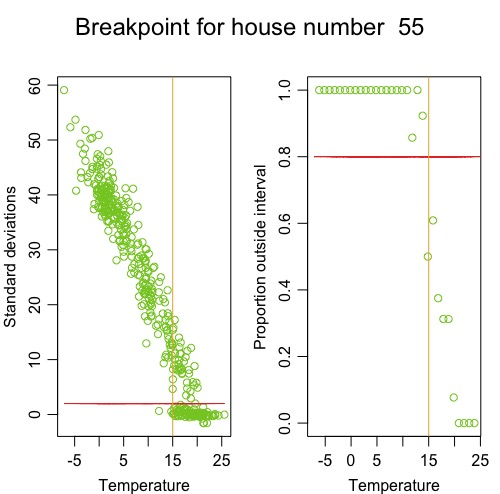
\includegraphics[width=0.8\textwidth]{../../../figures/Breakpoint.jpeg}
    \caption{An illustration of how the breakpoint is found using segmentation by significant deviations. On the left figure the line illustrates two standard deviations from the high temperature distribution.
    The right figure shows how many points are outside the two standard deviations. The last point below 80\% is the chosen breakpoint}
    \label{fig: Breakpoint}
\end{figure}

\begin{figure}
    \centering
    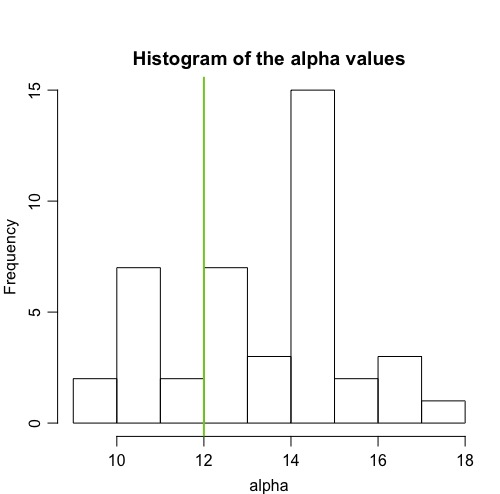
\includegraphics[width=0.8\textwidth]{../../../figures/AlphaHist.jpeg}
    \caption{A histogram of the alpha values for every house in the third segmentation method. The first quantile is chosen as the overall breakpoint. It is 12 degrees, illustrated by the green line}
    \label{fig: AlphaHist}
\end{figure}
